\section{System/Subsystem Design Description}



\subsection{System wide design decisions}
In dit hoofdstuk worden, zoals de tital al verraad, de design decisions behandeld. Hieronder vallen bijvoorbeeld
input/outputs van het systeem, gedrag keuzes en andere onderdelen die voor het gehele systeem gelden


\subsubsection*{Camera}
Aangezien het project inhoudt dat een aantal bijen gesimuleerd wordt, is het nodig om hun zintuigen ook te simuleren. Dit gebeurt door middel van een camera aan een raspberry pi. Hier zullen uiteraard eisen aan zitten, maar zullen in de SRS vermeldt worden. Om deze camera draadloos te laten werken is er ook een batterij pack nodig.

\subsubsection*{Server}
asd
\newline

\subsubsection*{Simulatie}
    \begin{center}
    \hspace*{-3.5cm}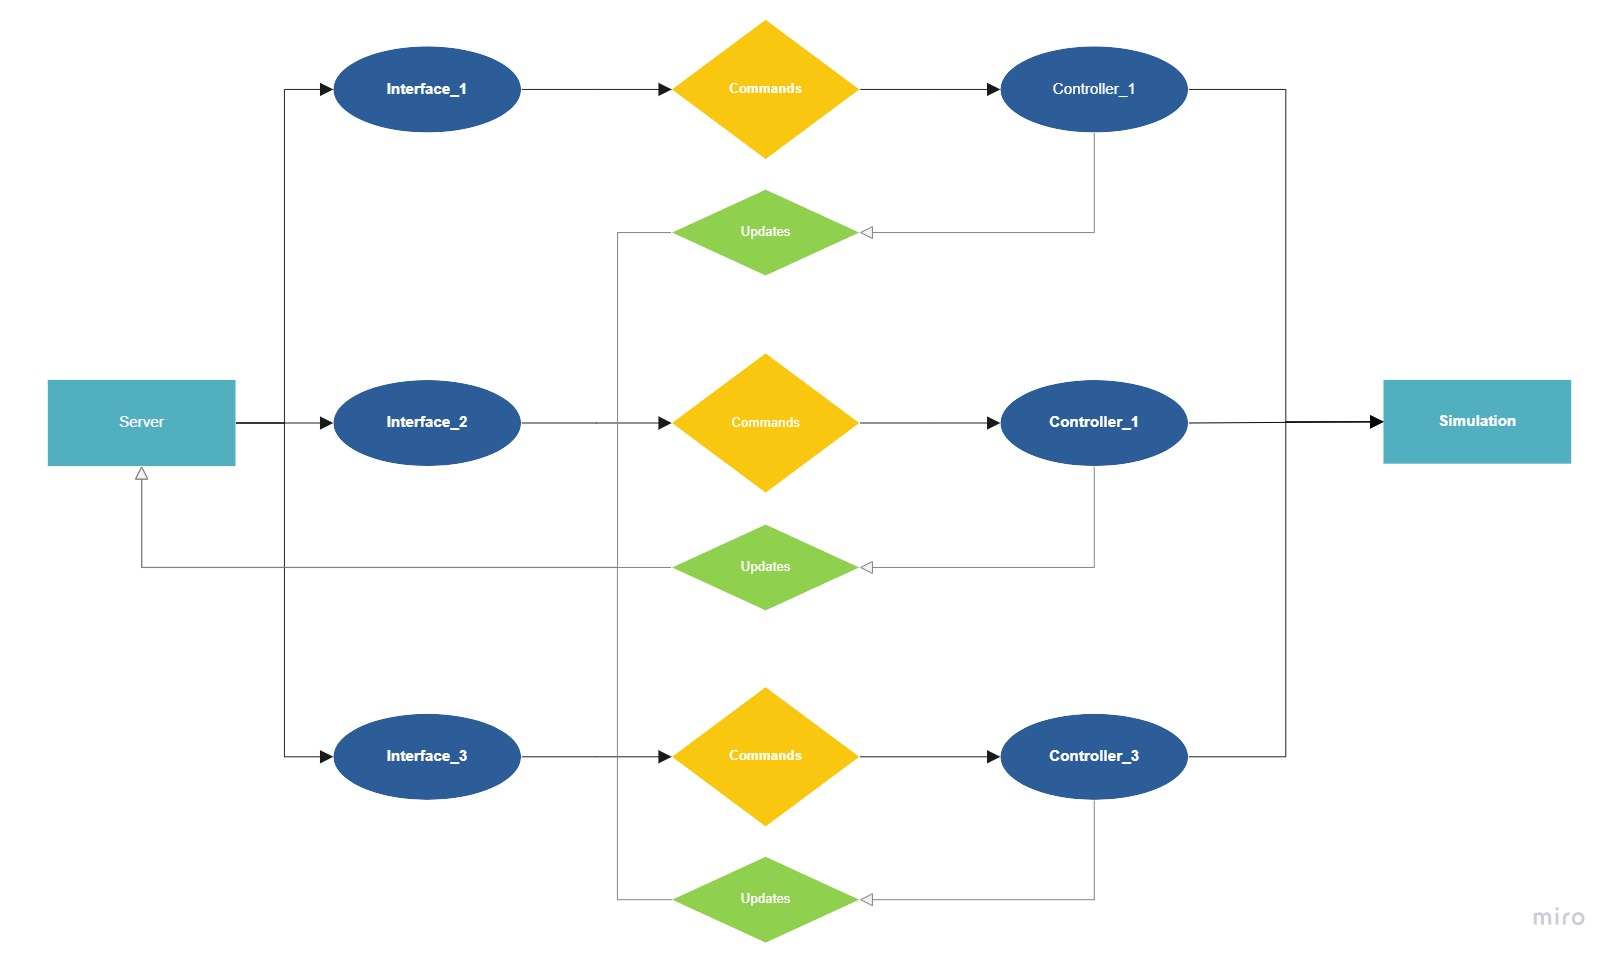
\includegraphics[width=1.6\textwidth]{../IMAGES/Simulation Interaction.jpg}
    \end{center}
    Het diagram hierboven weergeeft de communicatie tussen de simulatie en de server. In de simulatie
    wordt het gedrag van bijen met behulp van 3 ontworpen drones gesimuleerd. Om dat mogelijk te maken
    zijn voor de input en de output de volgende ontwerp keuzes gemaakt: \\

    \begin{description}\setlength{\itemindent}{0.1cm}
        \item[INPUT:] \hfill
        \begin{enumerate}
            \item De input voor de simulatie is altijd een opdracht naar een controller. Deze opdracht is een
            actie die een drone moet uitvoeren waarbij een positie meegegeven wordt  naarr de volgende verplaatsingsstap.
            Dit wordt mogelijk gemaakt door te communiceren tegen een opgebouwde interface. Deze
            interface communiceerd dan vervolgens tegen een controller die een gesimuleerde drone bestuurd.
        \end{enumerate}
        \newpage
        \item[OUTPUT:] \hfill
        \begin{enumerate}
            \item De output bij deze simulatie is verplaatsing van de gesimuleerde drone naar een geplannde positie.
            \item Daarnaast is er ook een andere continue output van de simulatie. Dat is een bericht die afkomstig
            is van een controller. Een controller stuurt om de bepaalde tijd een bericht naar de server met
            de informatie over de positie van de bestuurde drone.
        \end{enumerate}


    \end{description}

    \newpage
\subsection{System architectural design}
Uiteraard is het project een samenhangend geheel. Dit betekent dat er onderdelen zijn die afhankelijk zijn van andere onderdelen. Deze onderdelen zullen vermeld worden.

\subsubsection*{System components}
Diagram met hardware en software componenten van het gehelen systeem en de relatie tussen deze onderdelen < goeie, moeten we doen

Zoals op de afbeelding gebeeld wordt, is de camera afhankelijk van een raspberry pi. Dit komt omdat de beeld verwerkt moet worden door een microprocessor. Zo is er ook een samenhang tussen ...
